
\section{Appendix}

\begin{frame}

    \label{min_wage_plot}
    
    \frametitle{State minimum wage trends} % Title
    \framesubtitle{}  % Subtitle
    \rmfamily % Font
    
    \begin{wideitemize}
        \item States have been increasing their \textcolor{fblu}{minimum wage rates}, with varying intensity
    \end{wideitemize}

    \begin{center}
        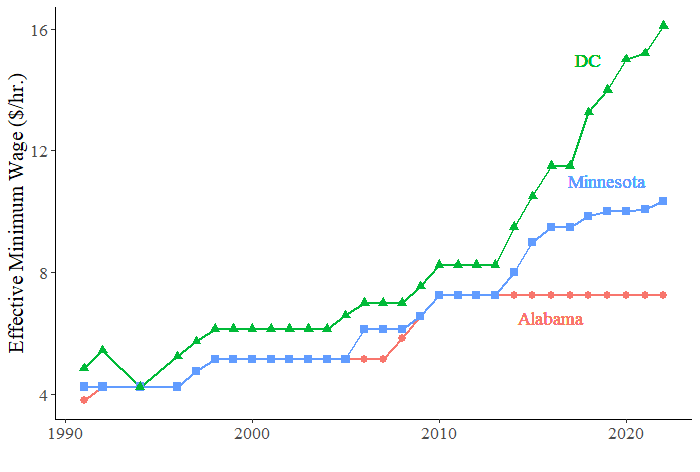
\includegraphics[scale=0.5]{min_wage_plot_simp.png}
    \end{center}
    
    \hyperlink{main_idea}{\beamerbutton{Back}}
    
\end{frame}

\begin{frame}

    \label{min_wage_plot_allstates}
    
    \frametitle{State minimum wage trends} % Title
    \framesubtitle{}  % Subtitle
    \rmfamily % Font
    
    \begin{wideitemize}
        \item States have been increasing their \textcolor{fblu}{minimum wage rates}, with varying intensity
    \end{wideitemize}

    \begin{center}
        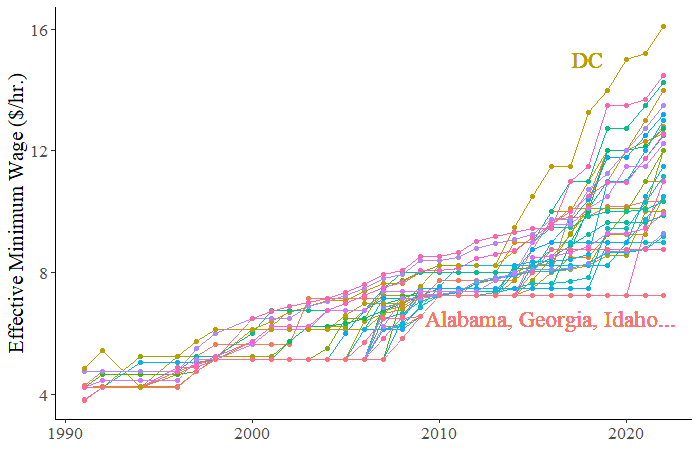
\includegraphics[scale=0.5]{min_wage_plot.png}
    \end{center}
    
    \hyperlink{main_idea}{\beamerbutton{Back}}
    
\end{frame}

\begin{comment}
\begin{frame}

    \label{quitting}
    \frametitle{Quitting decision I} % Title
    \framesubtitle{}  % Subtitle
    \rmfamily % Font

    \begin{wideitemize}
        \item Workers will quit opioids \textcolor{fblu}{if the expected utility of quitting is greater than the disutility of quitting} (\(\mathcal{C}_{quit}\))
        \item If the \textcolor{fblu}{minimum wage is not binding} and \textcolor{fblu}{the law is passed}
        \[
        q_{w_{it} > w^{min}_t} = \mathbbm{1}\{u\left(f(\theta_{it})L_{it}\right) - \mathcal{C}_{quit} \geq u\left(\left(f(\theta_{it}) - \kappa\right)L_{it}\right)\}
        \]
        \vspace{-15pt}
        \item If the \textcolor{fblu}{minimum wage is binding} and \textcolor{fblu}{the law is passed}
        \[
        q_{\,w_{it} = w^{min}_t} = \mathbbm{1}\{u\left(w^{min}_tL_{it}\right) - \mathcal{C}_{quit} \geq 0\}
        \]
    \end{wideitemize}
    
    \hyperlink{decision_making}{\beamerbutton{Back}}    

\end{frame}


\begin{frame}

    \frametitle{Quitting decision II} % Title
    \framesubtitle{}  % Subtitle
    \rmfamily % Font

    \begin{wideitemize}
        \item As long as
        \[
        u\left(f(\theta_{it})L_{it}\right) - u\left(\left(f(\theta_{it}) - \kappa\right)L_{it}\right) \geq \mathcal{C}_{quit} \geq u\left(w^{min}_tL_{it}\right)
        \]
        we should observe \textcolor{fblu}{more quitting where the minimum wage is less binding}
        \item This relation depends on \textcolor{fblu}{how much opioids affect productivity} and \textcolor{fblu}{how costly quitting is}
    \end{wideitemize}
    
    \hyperlink{decision_making}{\beamerbutton{Back}}    

\end{frame}
\end{comment}

\begin{frame}

    \label{perc_comparison_3}
    
    \frametitle{Percentiles comparison} % Title
    \framesubtitle{}  % Subtitle
    \rmfamily % Font

    \begin{center}
        \includegraphics[scale=0.4]{pmq10_lab_for_rate_comp6.png}
    \end{center}
    
    \hyperlink{lab_force_rate_result}{\beamerbutton{Back}}
    
\end{frame}

\begin{frame}

    \label{perc_comparison_31}
    
    \frametitle{Percentiles comparison} % Title
    \framesubtitle{}  % Subtitle
    \rmfamily % Font

    \begin{center}
        \includegraphics[scale=0.4]{pmq10_lab_for_rate_comp24.png}
    \end{center}
    
    \hyperlink{lab_force_rate_result}{\beamerbutton{Back}}
    
\end{frame}

\begin{frame}

    \label{perc_comparison_1}
    
    \frametitle{Percentiles comparison} % Title
    \framesubtitle{}  % Subtitle
    \rmfamily % Font

    \begin{center}
        \includegraphics[scale=0.4]{pmq10_unemp_rate_comp6.png}
    \end{center}
    
    \hyperlink{unemp_rate_result}{\beamerbutton{Back}}
    
\end{frame}

\begin{frame}

    \label{perc_comparison_12}
    
    \frametitle{Percentiles comparison} % Title
    \framesubtitle{}  % Subtitle
    \rmfamily % Font

    \begin{center}
        \includegraphics[scale=0.4]{pmq10_unemp_rate_comp24.png}
    \end{center}
    
    \hyperlink{unemp_rate_result}{\beamerbutton{Back}}
    
\end{frame}

\begin{frame}

    \label{perc_comparison_2}
    
    \frametitle{Percentiles comparison} % Title
    \framesubtitle{}  % Subtitle
    \rmfamily % Font

    \begin{center}
        \includegraphics[scale=0.4]{pmq10_emp_rate_comp6.png}
    \end{center}
    
    \hyperlink{emp_rate_result}{\beamerbutton{Back}}
    
\end{frame}

\begin{frame}

    \label{perc_comparison_21}
    
    \frametitle{Percentiles comparison} % Title
    \framesubtitle{}  % Subtitle
    \rmfamily % Font

    \begin{center}
        \includegraphics[scale=0.4]{pmq10_emp_rate_comp24.png}
    \end{center}
    
    \hyperlink{emp_rate_result}{\beamerbutton{Back}}
    
\end{frame}

\begin{frame}

    \label{ta_3}
    
    \frametitle{Time Averages} % Title
    \framesubtitle{}  % Subtitle
    \rmfamily % Font

    \begin{center}
        \includegraphics[scale=0.4]{pmq10_lab_for_rate_ta.png}
    \end{center}
    
    \hyperlink{lab_force_rate_result}{\beamerbutton{Back}}
    
\end{frame}

\begin{frame}

    \label{ta_1}
    
    \frametitle{Time Averages} % Title
    \framesubtitle{}  % Subtitle
    \rmfamily % Font

    \begin{center}
        \includegraphics[scale=0.4]{pmq10_unemp_rate_ta.png}
    \end{center}
    
    \hyperlink{unemp_rate_result}{\beamerbutton{Back}}
    
\end{frame}

\begin{frame}

    \label{ta_2}
    
    \frametitle{Time Averages} % Title
    \framesubtitle{}  % Subtitle
    \rmfamily % Font

    \begin{center}
        \includegraphics[scale=0.4]{pmq10_emp_rate_ta.png}
    \end{center}
    
    \hyperlink{emp_rate_result}{\beamerbutton{Back}}
    
\end{frame}

\begin{frame}

    \label{presc_3}
    
    \frametitle{Controlling for prescriptions} % Title
    \framesubtitle{}  % Subtitle
    \rmfamily % Font

    \begin{center}
        \includegraphics[scale=0.4]{pmq10_lab_for_rate_p.png}
    \end{center}
    
    \hyperlink{lab_force_rate_result}{\beamerbutton{Back}}
    \hyperlink{presc_indeff}{\beamerbutton{Individual effects}}

\end{frame}

\begin{frame}

    \label{presc_1}
    
    \frametitle{Controlling for prescriptions} % Title
    \framesubtitle{}  % Subtitle
    \rmfamily % Font

    \begin{center}
        \includegraphics[scale=0.4]{pmq10_unemp_rate_p.png}
    \end{center}
    
    \hyperlink{unemp_rate_result}{\beamerbutton{Back}}
    \hyperlink{presc_indeff}{\beamerbutton{Individual effects}}
    
\end{frame}

\begin{frame}

    \label{presc_2}
    
    \frametitle{Controlling for prescriptions} % Title
    \framesubtitle{}  % Subtitle
    \rmfamily % Font

    \begin{center}
        \includegraphics[scale=0.4]{pmq10_emp_rate_p.png}
    \end{center}
    
    \hyperlink{emp_rate_result}{\beamerbutton{Back}}
    \hyperlink{presc_indeff}{\beamerbutton{Individual effects}}
    
\end{frame}

\begin{frame}

    \label{presc_indeff}
    
    \frametitle{Prescription Effects} % Title
    \framesubtitle{}  % Subtitle
    \rmfamily % Font

    \begin{center}
        \includegraphics[scale=0.4]{pmq10_prescriptions.png}
    \end{center}
    
    \hyperlink{emp_rate_result}{\beamerbutton{Back}}
    
\end{frame}


\begin{frame}[shrink=5]

    \label{table_heroin}
    
    \frametitle{Heroin} % Title
    \framesubtitle{}  % Subtitle
    \rmfamily % Font

    \begin{table}[ht]
        \centering
        \begin{tabular}{lcccc}
        \toprule
         & \textbf{Estimate} & \textbf{Std. Error} & \textbf{t value} & \textbf{Pr(>|t|)} \\
        \midrule
        Intercept  & 5.600 & 2.135 & 2.623 & 0.0211 * \\
        Kaitz-0.10 & 9.613 & 5.021 & 1.914 & 0.0778 . \\
        \midrule
        \multicolumn{5}{l}{\textit{Signif. codes:  0 '***' 0.001 '**' 0.01 '*' 0.05 '.' 0.1 ' ' 1}} \\
        \midrule
        \multicolumn{5}{l}{\textbf{Residual standard error}: 1.95 on 13 degrees of freedom} \\
        \multicolumn{5}{l}{\textbf{Multiple R-squared}: 0.2199, \textbf{Adjusted R-squared}: 0.1599} \\
        \multicolumn{5}{l}{\textbf{F-statistic}: 3.665 on 1 and 13 DF, \textbf{p-value}: 0.07783} \\
        \bottomrule
        \end{tabular}
        %\caption{Regression Results}
        %\label{tab:regression_results}
    \end{table}
    
    \hyperlink{heroin_result}{\beamerbutton{Back}}
    
\end{frame}


\begin{frame}[shrink=5]

    \label{table_methadone}
    
    \frametitle{Methadone} % Title
    \framesubtitle{}  % Subtitle
    \rmfamily % Font

    \begin{table}[ht]
        \centering
        \begin{tabular}{lcccc}
        \toprule
         & \textbf{Estimate} & \textbf{Std. Error} & \textbf{t value} & \textbf{Pr(>|t|)} \\
        \midrule
        Intercept  & -0.4800 & 0.8021 & -0.598 & 0.560 \\
        Kaitz-0.10 & -0.6460 & 1.8900 & -0.342 & 0.738 \\
        \midrule
        \multicolumn{5}{l}{\textit{Signif. codes:  0 '***' 0.001 '**' 0.01 '*' 0.05 '.' 0.1 ' ' 1}} \\
        \midrule
        \multicolumn{5}{l}{\textbf{Residual standard error}: 0.7576 on 13 degrees of freedom} \\
        \multicolumn{5}{l}{\textbf{Multiple R-squared}: 0.008906, \textbf{Adjusted R-squared}: -0.06733} \\
        \multicolumn{5}{l}{\textbf{F-statistic}: 0.1168 on 1 and 13 DF, \textbf{p-value}: 0.738} \\
        \bottomrule
        \end{tabular}
        %\caption{Regression Results}
        %\label{tab:regression_results}
    \end{table}
    
    \hyperlink{heroin_result}{\beamerbutton{Back}}
    
\end{frame}


\begin{frame}[shrink=5]

    \label{table_otheropioids}
    
    \frametitle{Other opioids} % Title
    \framesubtitle{}  % Subtitle
    \rmfamily % Font

    \begin{table}[ht]
        \centering
        \begin{tabular}{lcccc}
        \toprule
         & \textbf{Estimate} & \textbf{Std. Error} & \textbf{t value} & \textbf{Pr(>|t|)} \\
        \midrule
        Intercept  & -3.486 & 2.530 & -1.378 & 0.192 \\
        Kaitz-0.10 & -7.537 & 5.949 & -1.267 & 0.227 \\
        \midrule
        \multicolumn{5}{l}{\textit{Signif. codes:  0 '***' 0.001 '**' 0.01 '*' 0.05 '.' 0.1 ' ' 1}} \\
        \midrule
        \multicolumn{5}{l}{\textbf{Residual standard error}: 2.31 on 13 degrees of freedom} \\
        \multicolumn{5}{l}{\textbf{Multiple R-squared}: 0.1099, \textbf{Adjusted R-squared}: 0.04143} \\
        \multicolumn{5}{l}{\textbf{F-statistic}: 1.605 on 1 and 13 DF, \textbf{p-value}: 0.2274} \\
        \bottomrule
        \end{tabular}
        %\caption{Regression Results}
        %\label{tab:regression_results}
    \end{table}
    
    \hyperlink{heroin_result}{\beamerbutton{Back}}
    
\end{frame}

\begin{frame}[shrink=5]

    \label{table_othersync}
    
    \frametitle{Other synthetic opioids} % Title
    \framesubtitle{}  % Subtitle
    \rmfamily % Font

    \begin{table}[ht]
        \centering
        \begin{tabular}{lcccc}
        \toprule
         & \textbf{Estimate} & \textbf{Std. Error} & \textbf{t value} & \textbf{Pr(>|t|)} \\
        \midrule
        Intercept  & 4.944 & 5.995 & 0.825 & 0.424 \\
        Kaitz-0.10 & 8.056 & 14.097 & 0.571 & 0.577 \\
        \midrule
        \multicolumn{5}{l}{\textit{Signif. codes:  0 '***' 0.001 '**' 0.01 '*' 0.05 '.' 0.1 ' ' 1}} \\
        \midrule
        \multicolumn{5}{l}{\textbf{Residual standard error}: 5.475 on 13 degrees of freedom} \\
        \multicolumn{5}{l}{\textbf{Multiple R-squared}: 0.0245, \textbf{Adjusted R-squared}: -0.05053} \\
        \multicolumn{5}{l}{\textbf{F-statistic}: 0.3266 on 1 and 13 DF, \textbf{p-value}: 0.5774} \\
        \bottomrule
        \end{tabular}
        %\caption{Regression Results}
        %\label{tab:regression_results}
    \end{table}
    
    \hyperlink{heroin_result}{\beamerbutton{Back}}
    
\end{frame}


\begin{frame}

    \label{github_link}
    
    \frametitle{Code} % Title
    \framesubtitle{}  % Subtitle
    \rmfamily % Font
    
    \begin{center}
        \href{https://github.com/guillelozabala/masters_thesis}{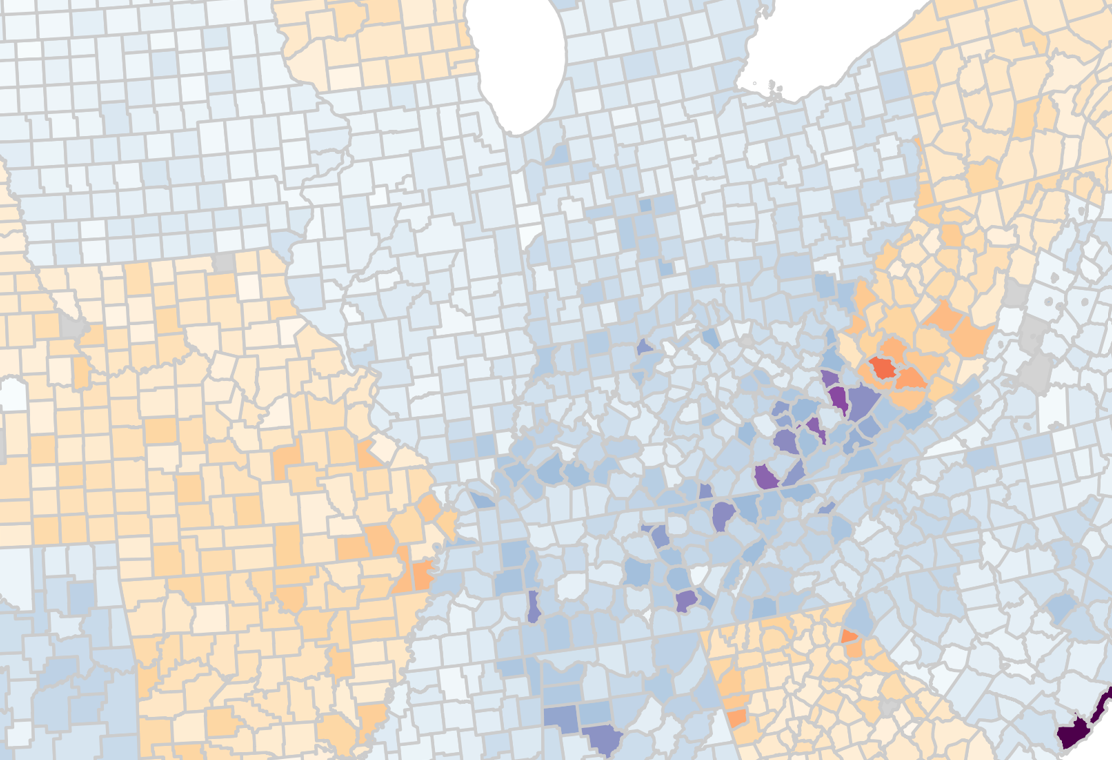
\includegraphics[scale=0.4]{thumbnail.png}}
    \end{center}
    
    %\hyperlink{}{\beamerbutton{Back}}
    
\end{frame}

